%!TEX program = xelatex

\documentclass[compress]{beamer}
%--------------------------------------------------------------------------
% Common packages
%--------------------------------------------------------------------------
\usepackage[english]{babel}
\usepackage{pgfpages} % required for notes on second screen
\usepackage{graphicx}

\usepackage{multicol}
\usepackage{url}

\usepackage{tabularx,ragged2e}
\usepackage{booktabs}


%--------------------------------------------------------------------------
% Load theme
%--------------------------------------------------------------------------
\usetheme[basicfont]{hri}

\usepackage{dtklogos} % must be loaded after theme
\usepackage{tikz}
\usetikzlibrary{calc,mindmap,backgrounds,positioning}

\graphicspath{{figs/}}
\setbeamercolor{refToContribCol}{bg=hriSec1Comp,fg=white}
\newcommand{\refToContrib}[1]{%
    \begin{beamercolorbox}[wd=\linewidth,ht=2ex,dp=0.7ex]{refToContribCol}%
    \hspace{0.5em}$\hookrightarrow$ #1%
    \end{beamercolorbox}%
}%

%--------------------------------------------------------------------------
% General presentation settings
%--------------------------------------------------------------------------
\title{Cognitive Architectures?}
\subtitle{Q1 -- Why should you use cognitive architectures - how would they
benefit your research as a theoretical framework, a tool and/or a methodology?}
\date{7th March 2016\\ {\tiny \url{https://sites.google.com/site/cogarch4socialhri2016/}}}
\author{}
\institute{
\includegraphics[height=15mm]{plymouth-logo}}
%\\Centre for Robotics \& Neural
%Systems\\{\Medium Plymouth University}}

%--------------------------------------------------------------------------
% Notes settings
%--------------------------------------------------------------------------
%\setbeameroption{show notes on second screen}

\begin{document}
%--------------------------------------------------------------------------
% Titlepage
%--------------------------------------------------------------------------

\maketitle

%\imageframe[Children playing with\\the Ranger robot]{photo-fullscreen.jpg}
%\imageframe{photo-fullscreen.jpg}


\begin{frame}{Three Interpretations of CogArch}

    \begin{multicols}{2}
        \resizebox{0.7\columnwidth}{!}{%
            \begin{tikzpicture}[
                    >=latex,
                every edge/.style={<-, draw, very thick}]

            \path[small mindmap, 
                level 1 concept/.append style={sibling angle=360/6}, 
                level 2 concept/.append style={sibling angle=60}, 
            concept color=hriSec1,text=white]
            node[concept] {Cognitive Architectures}
                [clockwise from=60]
                child[concept color=hriSec3Dark,text=white] { node[concept]{1. Model} }
                child[concept color=hriSec2Dark,text=white] { node[concept]{2. Integration} }
                child[concept color=hriSec2CompDark,text=white] { node[concept] {3. Methodology}};


        \end{tikzpicture}
    }
    \vfill
    \columnbreak

    {\Medium 1. Models of Human Cognition}

    {\scriptsize -- Modelling (aspects of) human cognition \\-- Subsequent application to robots}

    {\Medium 2. Technical Integration}

    {\scriptsize -- Define required functionality of robots \\-- Implement algorithms (etc) necessary}

    {\Medium 3. CogArch as Methodology}

    {\scriptsize -- Formalising assumptions \\-- Integrating knowledge from multiple disciplines \\-- Iteratively updating architecture}

    %\refToContrib{Someone here...}

    \end{multicols}
\end{frame}

\begin{frame}{1. Models of Human Cognition}    

    \begin{itemize}
        \item Model some human cognitive phenomenon, or preferably set of phenomena (typically based on human behavioural data)
        \item Derive operating principles/algorithms that fulfil the requirements of the human behaviour
        \item Verify/validate resulting model by fitting to existing human data, or making predictions of human behaviour
        \item Apply model to robotics system
    \end{itemize}
    
    Multiple examples in the literature of (aspects of) this process.

\end{frame}


\begin{frame}{1. Models of Human Cognition}    

    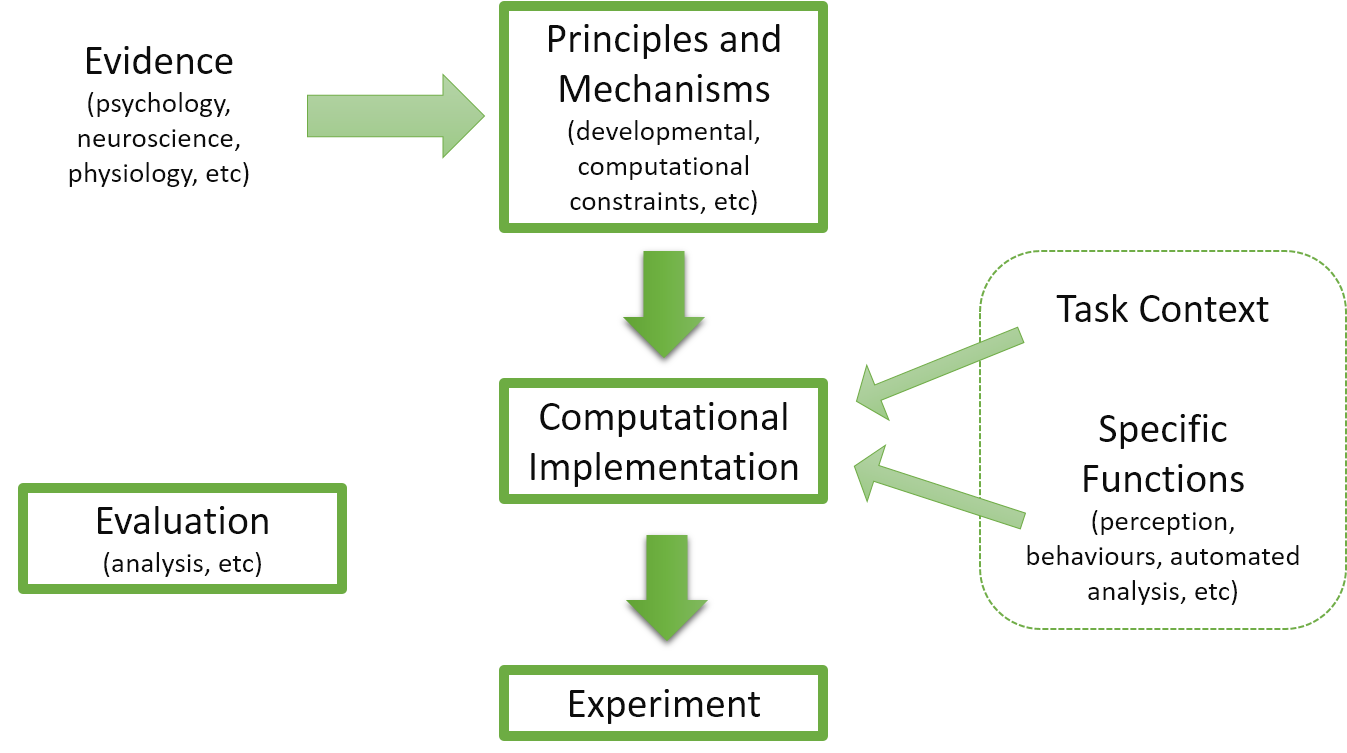
\includegraphics[height=60mm]{cogarch-cognitive-integration}

\end{frame}


\begin{frame}{Architectures to model human cognition}

\resizebox{!}{0.7\paperheight}{%
\tikzset{subpart/.style={draw, font=\scriptsize, fill opacity=0.5, text opacity=1, fill=white!50}}
\begin{tikzpicture}[
    >=latex,
    node distance=1.5,
    every edge/.style={draw, very thick},
    skill/.style={draw, rounded corners, align=center, inner sep=5pt, fill=black!20},
    stmt/.style={align=center, font=\Medium},
    label/.style={midway, align=center, font=\scriptsize, fill=white}]

    \node at (0,0)[skill, fill=hriSec2!50] (a1) {Shared Plan Elaboration};

    \node [skill, fill=hriSec2!50,above=of a1] (a2) {Intention Prediction};
    \node [skill, fill=hriSec2!50,left=of a1] (a3) {Mental State Management};
    \node [skill, fill=hriSec2!50,right=of a1] (a4) {Communication for\\Joint Action};
    \node [skill, fill=hriSec2!50,below=of a1] (a5) {Shared Plan Achievement};
    \node [skill, fill=hriSec2!50,left=of a5] (a6) {Situation Assessment};


    \node [skill, fill=hriSec3!50,below left=of a5,anchor=north] (a7) {Action Achievement};
    \node [skill, fill=hriSec3!50,below right=of a5,anchor=north] (a8) {Human Action Monitoring};
  
    \node[below=3.7 of a5] (a14) {Human-aware geometric and task planners, real-time controllers, sensors...};

  \coordinate[below=3 of a6] (a9);

  \node[rotate=90,left=0.7 of a3.west] (distal) {\Medium\large DISTAL};
  \node[rotate=90] at (distal |- a7.south) {\Medium\large PROXIMAL};
  \node[rotate=90] at (distal |- a14) {\Medium\large MOTOR};

  \coordinate (a11) at (a9 -| distal.north);
  \coordinate (a12) at (a9 -| a4.east);
  \draw[dotted, thick] (a11) -- (a12);


  \coordinate (a13) at ($(a5)!0.5!(a7)$);
  \draw[dotted, thick] (a13 -| distal.north) -- (a13 -| a4.east);


  %%% Relations between components
  \path (a2) edge [->] node[label] {goal to execute} (a1);
  \path (a1) edge [->] node[label] {plan} (a5);
  \path (a2) edge [<-] node[label] {goal (order)} (a4);

  \path (a3) edge [<->, bend left=40, looseness=1.2] node[label,pos=0.1] {mental state information} (a4);
  \path (a3) edge [<->] (a2);
  \path (a3) edge [<->] (a1);
  \path (a3) edge [<->] (a5);

  \path (a6) edge [->] node[label] {conceptual\\world state} (a3);

  \path (a5) edge [<->] node[label] {coordination} (a4);

  \path (a5) edge [<->] node[label,right=0.5] {anchoring of actions} (a7);
  \path (a5) edge [<->] (a8);

  \path (a9) edge [->] node[label] {sensors} (a6);

  \coordinate (a10) at (a9 -| a7);
  \path (a10) edge [<->] node[label] {planning and control} (a7);

  \coordinate (a10) at (a9 -| a8);
  \path (a10) edge [<->] node[label] {sensors} (a8);

  \path (a7) edge [<->] node[label] {coordination} (a8);
 
\end{tikzpicture}
}

\begin{flushright}
\scriptsize \refToContrib{From Sandra's contribution}
\end{flushright}

\end{frame}


\begin{frame}{2. Technical Integration}    

    \begin{itemize}
        \item Start with the application domain/problem to be solved
        \item Define set of algorithms required to fulfil task
        \item Implement architecture on robot
        \item Run experiment
    \end{itemize}
    
	A few examples in the literature of (aspects of) this process.

\end{frame}

\begin{frame}{2. Technical Integration}    

    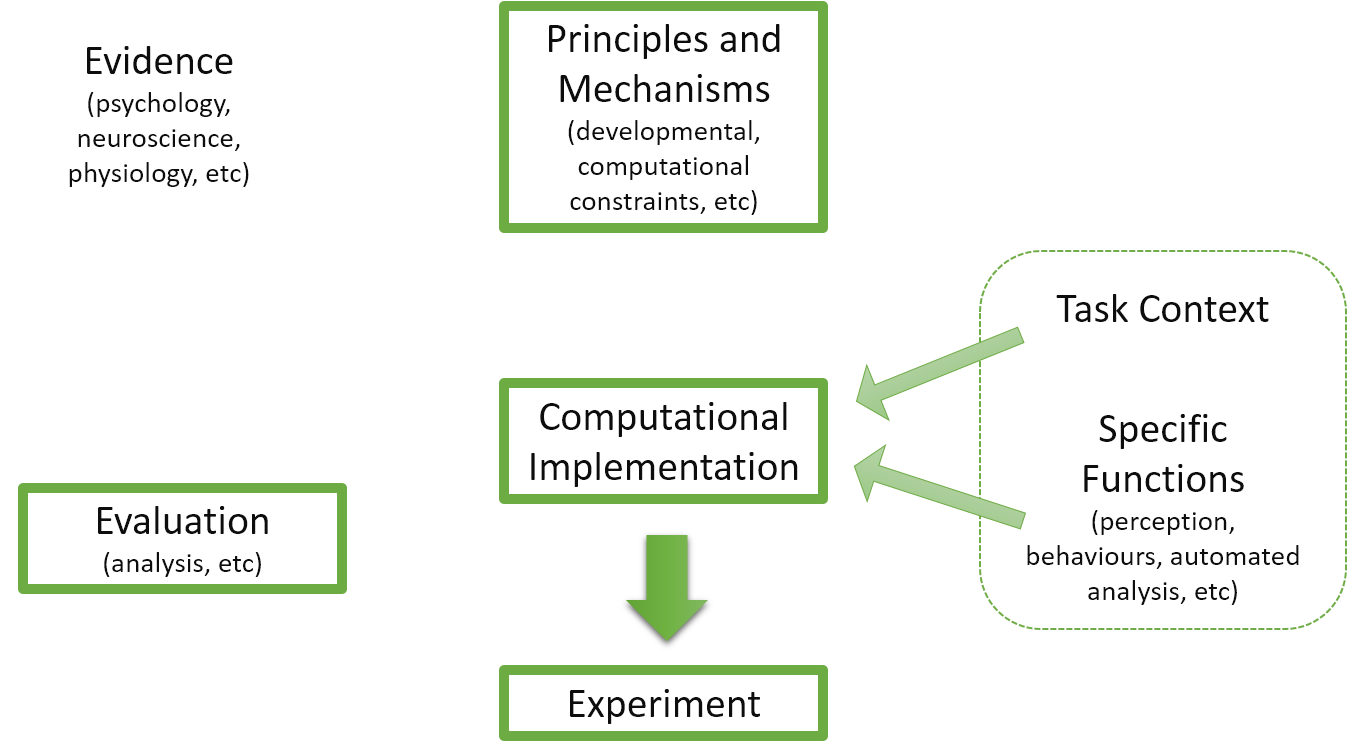
\includegraphics[height=60mm]{cogarch-technical-integration}

\end{frame}


\begin{frame}{3. CogArch as Methodology}    

    \begin{itemize}
        \item Human-derived evidence (from perhaps multiple domains)
        \item Define set of principles and constraints
        \item Implement architecture on robot; run experiment(s)
        \item Feed back results into principles and constraints; repeat
    \end{itemize}
    
    This process not typically explicit in the literature, but rather implicit in the development of cognitive (model) architectures in psychology/CogSci for example.
    
\end{frame}

\begin{frame}{3. CogArch as Methodology}    

    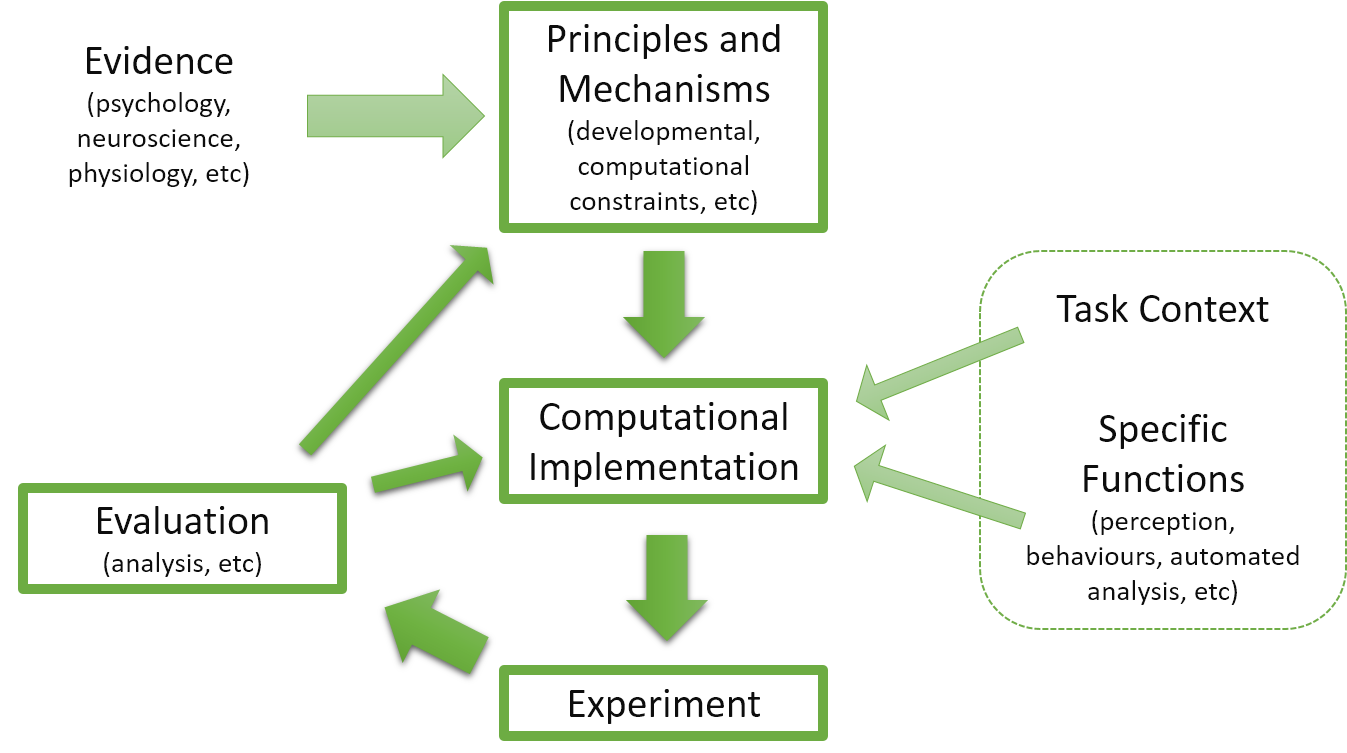
\includegraphics[height=60mm]{cogarch-methodology}

\end{frame}


\imageframe[Islands of desired Cognitive Functionality]{figs/islands1}{}
\imageframe[Linking islands together: the technical integration approach]{figs/islands2}{}
\imageframe[Exploring common underlying principles of the islands]{figs/islands3}{}
\imageframe[Constructing cognitive architectures from these principles]{figs/islands4}{}


\begin{frame}{Discussion: why use CogArch for social HRI?}
    

    \begin{itemize}
        \item ...
        \item ...
        \item ...
    \end{itemize}

    35 minutes of open discussion + 2 presentations

\end{frame}


\begin{frame}{Bibliography}
\begin{thebibliography}{10}

    \beamertemplatearticlebibitems
    \bibitem{lemaignan2015mutual}
    S. Lemaignan, P. Dillenbourg
    \newblock \doublequoted{Mutual Modelling: Inspiration for the Next Steps}
    \newblock 2015

    \beamertemplatearticlebibitems
    \bibitem{tenorth2010understanding}
    M. Tenorth, D. Nyga, M. Beetz
    \newblock \doublequoted{Understanding and Executing Instructions for Everyday Manipulation Tasks
    from the World Wide Web}
    \newblock 2010

    \beamertemplatearticlebibitems
    \bibitem{mavridis2015review}
    N. Mavridis
    \newblock \doublequoted{A review of verbal and non-verbal human–robot interactive communication}
    \newblock 2015



    \beamertemplatearticlebibitems
    \bibitem{kruijff2010situated}
    G.-J. M. Kruijff \emph{et al.}
    \newblock \doublequoted{Situated dialogue processing for human-robot interaction}
    \newblock 2010



  \end{thebibliography}
\end{frame}

\end{document}






